\documentclass[12pt]{report}
\usepackage[utf8]{inputenc}
\usepackage[portuguese]{babel}

\usepackage{graphicx}
\usepackage{tabularx}
\usepackage[section]{placeins}

\pagenumbering{arabic}

\begin{document}

  \begin{titlepage}
    \begin{center}
        \vspace*{1cm}
        
        \Huge
        \textbf{T05: Exploração de Marte}
        \vspace{0.5cm} \ \\
        \LARGE
        Agentes e Inteligência Artificial Distribuída
        
        \vfill
        
	
\includegraphics[width=0.6\textwidth]{FEUP_Logo}
	\break
        \small
        Novembro 2016
        
        \vfill
        
	\vspace{1.5cm}
        \normalsize{
	  Marina Camilo - up201307722 - up201307722@fe.up.pt \\
	  Diogo Ferreira - up201502853 - diogoff@fe.up.pt \\
	  Ângela Cardoso - up200204375 - angela.cardoso@fe.up.pt
        }
        
    \end{center}
  \end{titlepage}

\newpage
\tableofcontents

\clearpage
\chapter{Enunciado}

\section{Descrição do cenário}
No âmbito da unidade curricular de Agentes e Inteligência Artificial Distribuída, o nosso grupo propôs-se a implementar um Sistema Multi-Agente para simulação de um cenário de extração de minérios em Marte. Para tal, é necessário descobrir os minérios, extraí-los e transportá-los para a base. Sendo assim, no nosso sistema existem três tipos de Agentes:

\begin{itemize}
  \item \emph{Spotter} – Procura fontes de minérios e inspeciona-as para determinar se podem ser exploradoas. 
  \item \emph{Producer} – É chamado a uma fonte de minério por um \emph{spotter} para extrair o máximo de minério possível nessa fonte. 
  \item \emph{Transporter} – É alocado pelo \emph{producer} para carregar o minério obtido para a base.
\end{itemize}

De forma a facilitar a procura, todos os agentes podem localizar fontes de minérios e enviar a sua localização para os \emph{spotter} que os analisarão. A escolha do \emph{producer} por parte do \emph{spotter} segue um protocolo de negociação. A alocação dos \emph{transporters} a uma determinada fonte segue também um protocolo de negociação, iniciado pelo \emph{producer}. Esta alocação, terá em conta a quantidade de minério a transportar, de modo a determinar mais corretamente o número necessário de \emph{transporters}.

\section{Objectivos do trabalho}

Um dos objetivos deste trabalho é implementar os agentes de forma a que a simulação da exploração seja tão eficiente quanto possível. Para tal serão estudadas várias alternativas de implementação, de forma a determinar qual a melhor abordagem. No caso dos agentes do tipo \emph{spotter}, tencionamos usar algoritmos de distribuição do espaço a explorar entre eles, para que cubram toda a região mais rapidamente. Em relação aos \emph{producers} e \emph{transporters}, o objetivo é instalar protocolos de negociação que garantam que o melhor agente é escolhido para a tarefa.

\section{Resultados esperados e forma de avaliação}

Inicialmente serão implementadas apenas as funcionalidades básicas de cada Agente como tal:
A 1º fase de avaliação será verificar o sucesso da implementação do comportamento de cada agente. Após se garantir que todos os agentes realizam o seu papel corretamente passamos para a fase seguinte, a fase de implementação de restrições. 
Nesta 2º fase, irá avaliar–se se os \emph{transporters} chamados não ultrapassam a sua capacidade, se o \emph{transporters} chamados conseguem recolher todo o minério presente. 
Após estas fases, implementaremos algoritmos de forma a tornar mais eficiente esta demanda, avaliando se as alocações dos demais agentes correspondem ao mais disponível na altura. Se o mapa fica corretamente dividido entre os \emph{spotters} e se o tempo de simulação foi o mínimo para o caso em questão.

 
\chapter{Plataforma/Ferramenta}

\section{Para que serve}
  \subsection{Jade}
  Permite desenvolver agentes distruídos por \emph{containers} que podem estar em máquinas diferentes. Cada um destes agentes utiliza uma \emph{thread}. 

  \subsection{Repast 3}
  Permite construir simulações locais à máquina com diversos agentes. O processamento de cada agente é distribuído pelas \emph{threads}.

  \subsection{SAJaS}
  Junta estas duas plataformas e toma vantagem dos benefícios de ambas.

\section{Descrição das características principais}
  \subsection{Jade}
  Suporta troca de mensagens ACL que seguem a especificação FIPA e permite ter agentes remotos.
  
  \subsection{Repast 3}
  Suporta simulação de espaços físicos, representação 2D e 3D e análise em tempo real.

  \subsection{SAJaS}
  Permite manter o código exatamente igual apenas necessitando trocar as \emph{packages} usadas.

\section{Realce das funcionalidades relevantes para o trabalho}
Troca de mensagens no jade
Espaços no repast3
Scheduling no repast3

%escrever aqui

\chapter{Especificação}
%escrever aqui
\section{Identificação e caracterização dos agentes (arquitectura, comportamento, estratégias)}
%escrever aqui

\section{Protocolos de interacção}

\subsection{Divisão de espaços}
Inicialmente cada \emph{spotter} deve comunicar e acordar com os restantes \emph{spotters} o espaço reservado para este explorar.
É assumido que o espaço físico se trata sempre de uma matriz quadrada.

\begin{figure}[h]
  \centering
    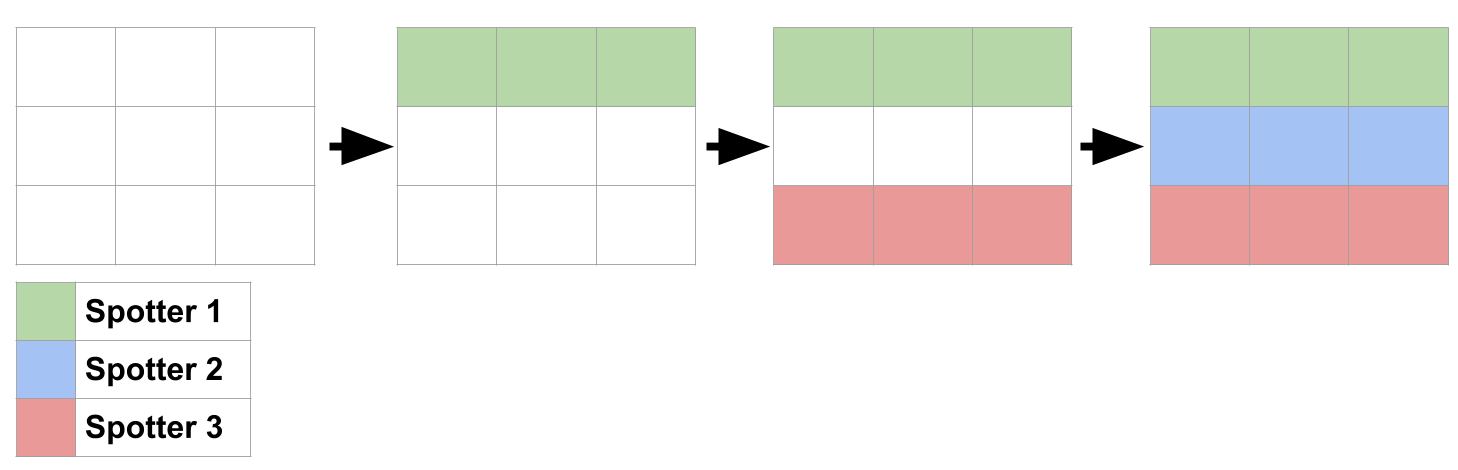
\includegraphics[width=0.6\textwidth]{spotter-spaces}
  \caption{\small{Alocação simples por linhas}}
\end{figure}

Inicialmente o espaço é divido por linhas e repartido pelos diferentes \emph{spotters}. Estes ficam encarregues de confirmar esta
afetação com os \emph{spotters} restantes.

\begin{figure}[h]
  \centering
    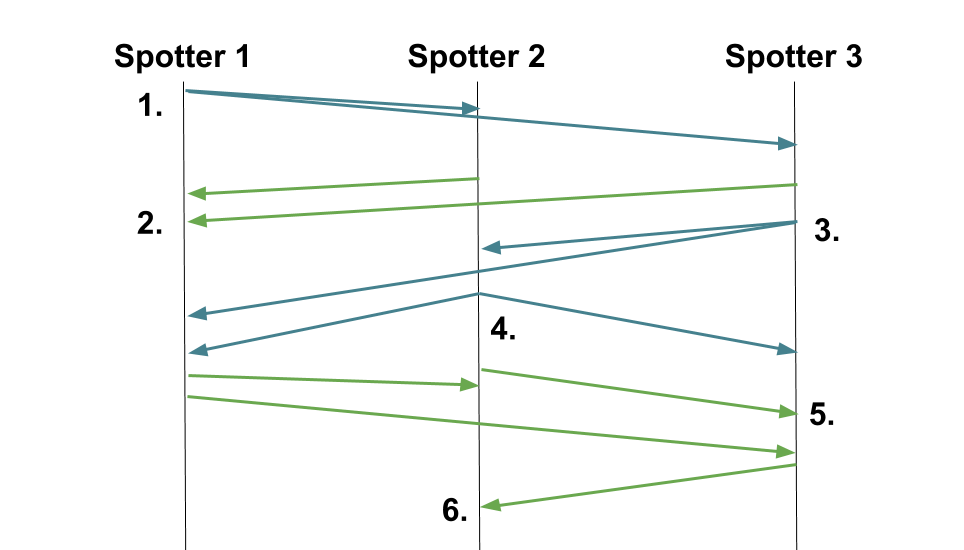
\includegraphics[width=0.6\textwidth]{spotter-agreement}
  \caption{\small{Diagrama temporal das comunicações entre \emph{spotters}}}
  
  \begin{enumerate}
    \item Spotter1 comunica ao restantes \emph{spotters} o espaço que este pretende explorar.
    \item Spotter1 recebe confirmação dos \emph{spotters} e fica afecto ao espaço que o mesmo pretendia.
    \item Spotter3 comunica ao restantes \emph{spotters} o espaço que este pretende explorar.
    \item Spotter2 comunica ao restantes \emph{spotters} o espaço que este pretende explorar.
    \item Spotter3 recebe confirmação dos \emph{spotters} e fica afecto ao espaço que o mesmo pretendia.
    \item Spotter2 recebe confirmação dos \emph{spotters} e fica afecto ao espaço que o mesmo pretendia.
  \end{enumerate}
\end{figure}

\FloatBarrier
\subsection{Afetação de Producers}
Uma vez encontrado minério é necessário chamar um \emph{producer} para o extrair. O \emph{spotter} envia então a posição do 
minério a todos os \emph{producers} e espera que lhe respondam com um valor indicante do esforço necessário a cada \emph{producer}.
O \emph{spotter} escolhe o \emph{producer} com o menor esforço e comunica de novo pedindo para confirmar a afetação do mesmo.
Caso seja recusado, porque o \emph{producer} foi afeto a outro minério entretanto, o \emph{spotter} pede de novo o valor do esforço
e repete o processo anterior.

Os \emph{producers} guardam numa \emph{queue} os diferentes minérios que vão extrair. Com esta \emph{queue} o calculo do esforço
para extrair um minério baseia-se em somar a distância entre cada um dos minérios, a distância do ponto corrente para o primeiro
minério e a distância do ultimo minério ao potencial minério.

\FloatBarrier
\subsection{Afetação de Transporters}
Após a extração do minério é necessário transportá-lo para a nave-mãe. O \emph{producer} que acabou de extrair o minério tem que selecionar 
um \emph{transporter}, do mesmo modo que o \emph{spotter} seleciona um \emph{producer}. Cada \emph{transporter} comunica o valor
do esforço e o minério que consegue transportar possibilitando o \emph{producer} de escalonar os diferentes agentes.

%escrever aqui
\section{Faseamento do projecto}

\begin{table}[htb]
\centering
\caption{Fases previstas para o projecto}
    \sffamily \begin{tabularx}{1.0\textwidth}{ p{3cm}  p{10,5cm} }
    \hline
    \textbf{1º Ponto} \hfill & Construir ambiente de simulação na tecnologia \emph{Repast} \\ \hline
    \textbf{2º Ponto} \hfill & Criação do \emph{spotter} com as função de explorar e dividir território a explorar. \\ \hline
    \textbf{3º Ponto} \hfill & Criação do \emph{producer} com a função básica de produzir. Melhoramento do \emph{spotter} para chamar \emph{producers}. \\ \hline
    \textbf{4º Ponto} \hfill & Criação do \emph{transporter} sem limite de capacidade e apenas com a função básica de transportar. Melhoramento do \emph{producer} para chamar \emph{transporters}. \\ \hline
    \textbf{5º Ponto} \hfill & Melhoria dos Agentes \emph{spotter}, \emph{producer} e \emph{transporter}. \\ \hline
    \textbf{6º Ponto} \hfill & Defenir estratégias de forma a tornar a exploração de Marte o mais eficiente possível. \\ \hline
    \end{tabularx} \normalfont
\end{table}

\chapter{Recursos}
%escrever aqui
\section{Bibliografia}
%escrever aqui
\section{Software}
%escrever aqui


\chapter{Exemplo Figura e tabela}

\begin{figure}[!htb]
\centering

\includegraphics[width=0.60\textwidth]{FEUP_Logo}
\caption[alguma coisa.]{Mais aluguma coisa} \label{fig:Array}
\end{figure}

\section{Baixando a partir de outro documento}

%
% Anexos
%
\appendix
\renewcommand{\chaptername}{Anexos}
\chapter{Anexos}
Dicas úteis e waypoints

\end{document}